%\documentclass[11pt]{article}
%\usepackage{fullpage}
%\usepackage{graphicx}

%\begin{document}

\subsection{Product perspective}
The TrackMe software-based service, Data4Help, has  other two services built on its top: AutomatedSOS and Track4Run. These two services exploit Data4Help's features, resources and links to external services. Not all the system's tasks in fact are provided only by the application: maps or payment services are committed to external systems. The application provides some services also for users who install it on a non-weareble device, but it mainly exploits weareble devices' features for all the three services. They are indeed based on health and location features that must be updated in real-time.\newline

A view of the relations that intervene among concepts that will be at the base of the system is given by the following diagram.\newline

\begin{center}
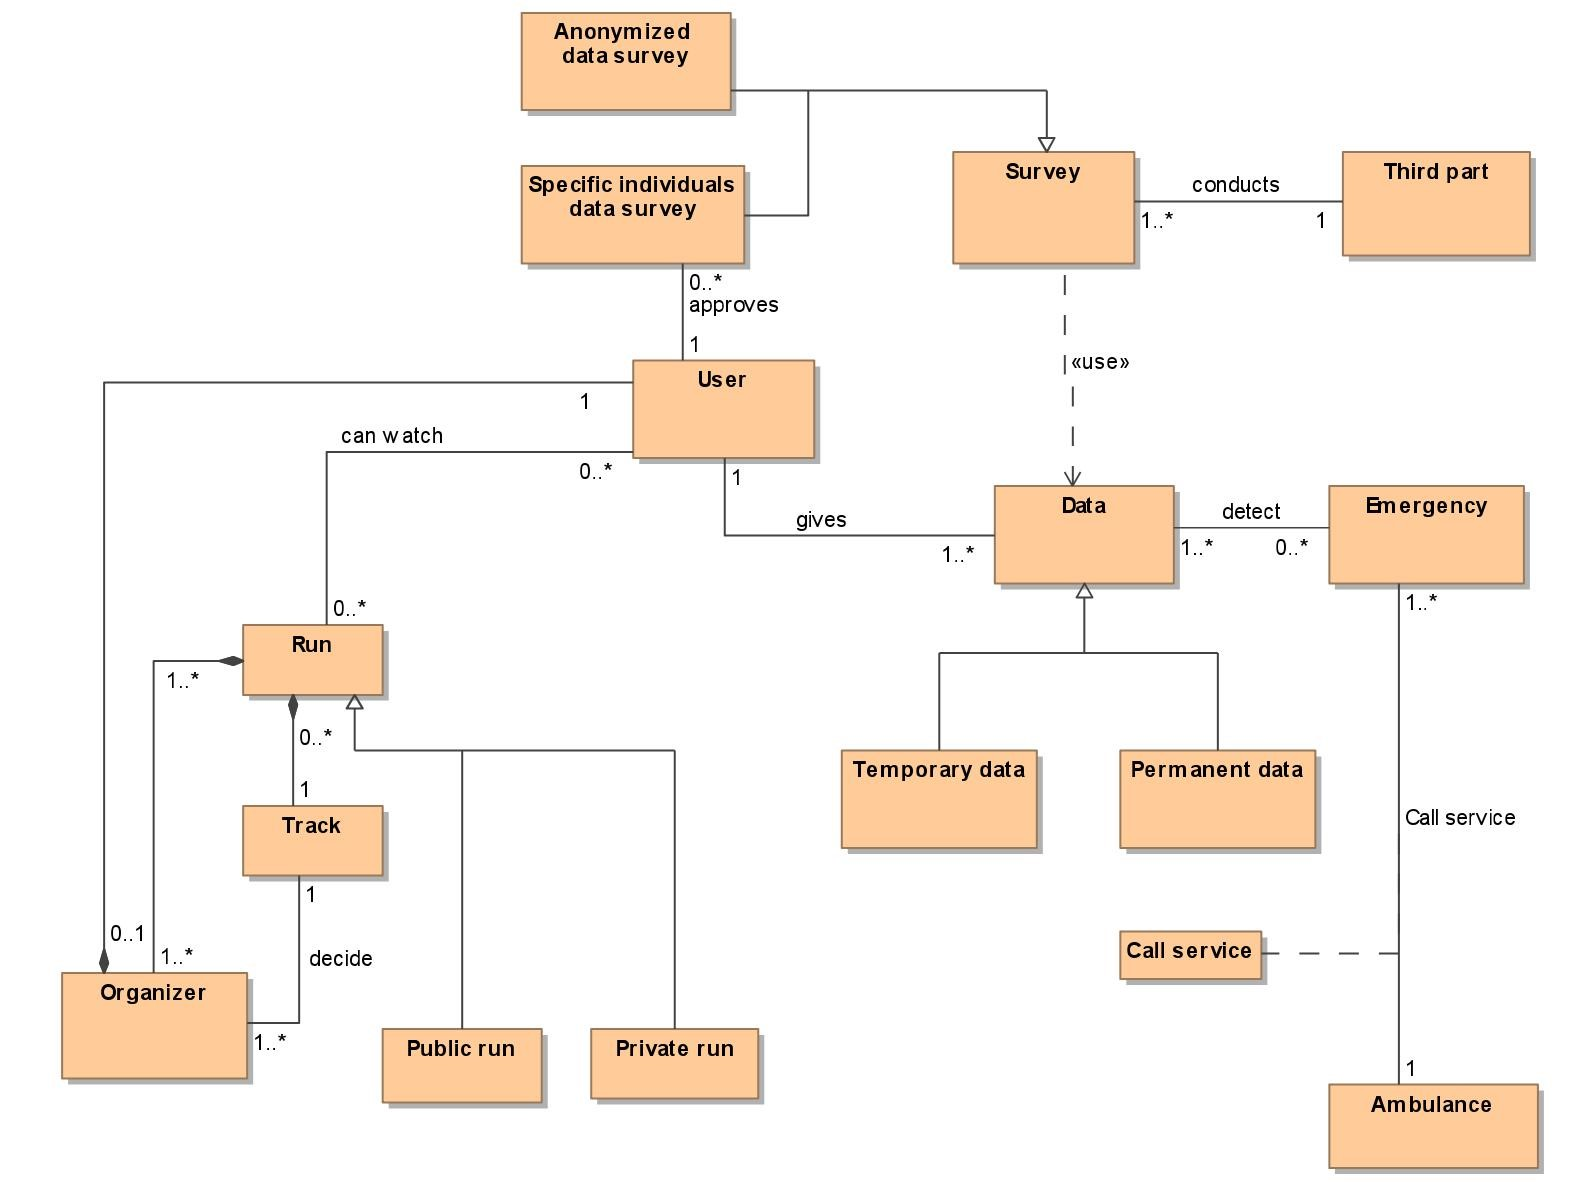
\includegraphics[scale=1]{sections/diagrams/class_diagram.jpg}
\end{center}

A central role is performed by data that can tell the user and third parties about his/her status. Besides data management(with a semi-passive role for the user), the application is about running races and allows persons to enter in contact with each other watching or organizing them. Finally, we can see different types of data, races and surveys, that requires different interactions with users.
\subsection{Product functions}
\subsection{User characteristics}
\subsection{Assumptions, dependencies and constraints}
%\end{document}
